\documentclass[12pt]{article}
\usepackage{geometry}                % See geometry.pdf to learn the layout options. There are lots.
\geometry{letterpaper}                   % ... or a4paper or a5paper or ...
%\geometry{landscape}                % Activate for for rotated page geometry
%\usepackage[parfill]{parskip}    % Activate to begin paragraphs with an empty line rather than an indent
\usepackage{graphicx}
\graphicspath{{images/}}
\usepackage{amsmath,amssymb,amsfonts,amsthm}
\usepackage{epstopdf}
\usepackage{epigraph}

% Computer Concrete
%\usepackage{concmath}
%\usepackage[T1]{fontenc}

% Times variants
%
\usepackage{mathptmx}
\usepackage[T1]{fontenc}
%
%\usepackage[T1]{fontenc}
%\usepackage{stix}
%
% Needs to typeset using LuaLaTeX:
%\usepackage{unicode-math}
%\setmainfont{XITS}
%\setmathfont{XITS Math}

\DeclareGraphicsRule{.tif}{png}{.png}{`convert #1 `dirname #1`/`basename #1 .tif`.png}

\theoremstyle{plain}
\newtheorem{theorem}{Theorem}
\newtheorem{corollary}[theorem]{Corollary}
\newtheorem{lemma}[theorem]{Lemma}
\newtheorem{proposition}[theorem]{Proposition}
\newtheorem{conjecture}[theorem]{Conjecture}
\newtheorem{question}[theorem]{Question}

\theoremstyle{definition}
\newtheorem{definition}[theorem]{Definition}
\newtheorem{example}[theorem]{Example}
\newtheorem*{keywords}{Keywords}

\theoremstyle{remark}
\newtheorem{remark}[theorem]{Remark}
\newtheorem{note}[theorem]{Note}

\newcommand{\defeq}{\overset{\mathrm{def}}{=}}

\title{Machine Learning Notes}
\author{Nhan Trong}
\date{\today}                                           % Activate to display a given date or no date

\begin{document}
\maketitle

\epigraph{Detective Spooner. \textit{Can a robot write a symphony? Can a robot turn a canvas into a beautiful masterpiece?} \\ Robot. \textit{Can you?}}{I, Robot}

\begin{note}
Refer to assignment PDF's. We'll use the usual subscript indexing notation instead of superscript like the lecture.
\end{note}

\part{Ex 8. Anomaly Detection and Recommender Systems}

\begin{keywords}
Collaborative filtering, cost function, gradient, regularization.
\end{keywords}

\section{Collaborative Filtering Learning Algorithm}

Let $n_m$ be the number of movies, $n_u$ be the number of users. Given rating matrix $Y$ and a number $n$, we want to find a feature matrix $X$ of size $n_m \times n$ and parameter matrix $\Theta$ of size $n_u \times n$, where the $i$-th row of $X$ represents the feature vector for the $i$-th movie, and the $j$-th row of $\Theta$ represents the parameter vector for the $j$-th user. In this context, $n$ represents the number of hidden dimensions of a movie, e.g. $X_{ik}$ could refer to say how much action movie $i$ has, $X_{il}$ could refer to how much romance it has, and so on. Similarly, $\Theta_{jk}$ would refer to how much user $j$ likes action, $\Theta_{jl}$ how much they like romance.

\begin{note}
These are only example features, since in fact we don't know what features the algorithm will pick up given rating matrix $Y$. The features learned might have nothing to do with common movie genres, for example.
\end{note}

\begin{question}
Can we cross validate to choose the best value $n$ for the number of hidden features?
\end{question}

\section{Cost Function and Gradient}

\begin{definition}
Define the collaborative filtering cost function to be the squared error over all parameters $\Theta$ and features $X$:
$$J(X, \Theta) = \frac{1}{2} \sum_{i,j:R_{ij}=1} (\Theta_j \cdot X_i - Y_{ij})^2.$$ 
\end{definition}

Then the partial derivatives of $J$ with respect to $x$ and $\theta$ are: 
\begin{align*}
\frac{\partial J}{\partial X_{ik}} &= \sum_{j:R_{ij}=1} (\Theta_j \cdot X_i - Y_{ij}) \Theta_{jk} \\
\frac{\partial J}{\partial \Theta_{jk}} &= \sum_{i:R_{ij}=1} (\Theta_j \cdot X_i - Y_{ij}) X_{ik}.
\end{align*}
The vectorized forms are surprisingly simple:
\begin{align*}
D &\defeq R * (X \Theta^T - Y) \\
J &= \frac{1}{2}D \cdot D \\
\frac{\partial J}{\partial X} &= D \Theta \\
\frac{\partial J}{\partial \Theta} &= D^T X,
\end{align*}
where $\cdot$ denotes the Frobenius inner product (just a natural extension of the vector dot product to matrices), and $*$ denotes element-wise multiplication. We need to multiply element-wise by $R$ to reduce $X\Theta^T - Y$ to elements where the corresponding entries in $Y$ are nonzero, because the summation is only over $i,j$ such that $R_{ij} = 1$, i.e. where $Y_{ij}$ is nonzero.

\section{Cost Function and Gradient with Regularization}

With regularization, the cost function and partials are: 
\begin{align*}
D &\defeq R * (X \Theta^T - Y) \\
J &= \frac{1}{2}D \cdot D + \frac{\lambda}{2} X \cdot X + \frac{\lambda}{2} \Theta \cdot \Theta \\
\frac{\partial J}{\partial X} &= D \Theta + \lambda X \\
\frac{\partial J}{\partial \Theta} &= D^T X + \lambda \Theta.
\end{align*}

\part{Week 10. Large Scale Machine Learning}

\begin{keywords}
Online learning, predicted CTR / click through rate, map-reduce, Hadoop.
\end{keywords}

\begin{question}
Can you use, say, Hadoop map-reduce for any generic processing task, e.g. parallel video transcoding?
\end{question}

\part{Week 11. Application: Photo OCR}

\begin{keywords}
Photo OCR vs scanned text OCR, text detection, bounding box expansion, character segmentation, character classification, pedestrian detection, sliding window detection, step size / stride, artificial data synthesis, data amplification, ceiling analysis.
\end{keywords}

\section{Photo OCR Pipeline}

\centerline{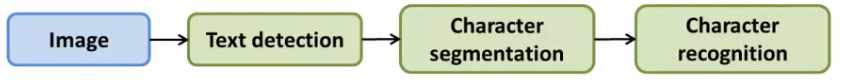
\includegraphics[width=1.0\textwidth]{ocrpipeline}}

\end{document}
